\documentclass[11pt,fleqn]{article}

\usepackage{graphicx}

\hoffset=-0.06\textwidth
\textwidth=1.12\textwidth
\voffset=-0.06\textheight
\textheight=1.12\textheight

%%%%%%%%%%%%%%%%%%%%%%%%%%%%%%%%%%%%%%%%%%%%%%%

\def\n{\noindent}
\def\dis{\displaystyle}

\def\bea{\begin{eqnarray}}
\def\nn{\nonumber\\}
\def\eea{\end{eqnarray}}
\def\beq{\begin{equation}}
\def\eeq{\end{equation}}


\def\wt#1{\widetilde{#1}}
%\def\wtt#1{\widetilde{\widetilde{#1}}}

\def\P{{\bf P}}
\def\a{{\bf a}}
\def\E{{\cal E}}
\def\D{{\bf D}}
\def\G{{\bf G}}
\def\u{{\bf u}}
\def\r{{\bf r}}
\def\k{{\bf k}}

\def\eps{\epsilon}
\def\epso{\eps_0}

\def\O{\Omega}
\def\Oo{\Omega_0}

\def\bc{_{\rm c}}
\def\veps{\varepsilon}

\def\half{{\textstyle{1\over2}}}

\def\ABINIT{{{\tt ABINIT}}}
\def\ANADDB{{\tt ANADDB}}
\def\DDB{{\tt DDB}}

%%%%%%%%%%%%%%%%%%%%%%%%%%%%%%%%%%%%%%%%%%%%%%%

\begin{document}

\begin{center}
{\Large\bf
Systematic second-order perturbation theory\\
\baselineskip 20pt
for displacements, strains, and electric fields
}
\large
\par\bigskip
Notes relevant to the {\tt ANADDB} module of {\tt ABINIT}
\par\medskip
D. Vanderbilt\\
\today
\end{center}


\bigskip
These notes were originally written to explain the background,
establish the notation, and provide an explanation of certain
features added to the \ANADDB\ \cite{abi} package in an upgrade implemented by
Xifan Wu in January 2004, providing for improved flexibility in the
computation of dielectric, elastic, piezoelectric, and related
tensors.  However, I believe they may prove helpful more generally,
e.g., as a starting point for the definition and computation of
higher-order derivatives, or of properties computed under conditions
of finite electric fields.

These notes will normally reside in the file {\sl `vanderbilt-anaddb-notes.pdf'}
in the {\sl `/Infos'} subdirectory of the \ABINIT\ distribution \cite{abi}.
Regarding the definitions of elastic tensors, especially under
conditions of finite pressure or stress, please also consult
the notes {\sl `elasticity-oganov.pdf'} \cite{oganov} written by A.~Oganov
and located in the same subdirectory.

I would like to thank X.~Wu, D.R.~Hamann, and K.M.~Rabe for input
and helpful comments.

%==============================================================
\section{Introduction}
%==============================================================

The purpose of these notes is to provide a systematic framework for
the discussion of response tensors that can be defined in terms of
three kinds of homogeneous perturbations in crystalline insulators:
\begin{itemize}
\item Zone-center phonons
\item Homogeneous electric fields
\item Homogeneous strains
\end{itemize}
In particular, the notes provide a set of definitions of many of
the elastic, dielectric, piezoelectric, and other tensors that
can be defined in terms of the system response to these
perturbations, and clarifies the connections between them.
In addition, the notes make a direct connection with the quantities
(i.e., the matrices of second derivatives) that are calculated and
stored in the ``derivative database'' (\DDB) of the
\ABINIT\ computer package, and with the analysis
of these carried out by the \ANADDB\ package of \ABINIT\
\cite{abi}.

%==============================================================
\section{Units}
%==============================================================

SI units are used throughout.  This is the convention of most
textbooks and review articles such as Lines and Glass \cite{lines},
Nye \cite{nye}, Ballato \cite{ballato}, etc.  However, Waghmare's
article \cite{waghmare}, and much of the usual electronic
structure literature, uses Gaussian units.  We recall here that in
SI units, potential = $(1/4\pi\epso)\,q_1q_2/r$, energy density =
$(\epso/2)\E^2$, and $D=\epso\,\E+P$.

%==============================================================
\section{Notation}
%==============================================================
\label{sec:notation}

Consider an insulating crystal with $N$ atoms per primitive cell.
We choose a reference state in which the lattice vectors are
${\bf a}_1$, ${\bf a}_2$, and ${\bf a}_3$ and the atomic coordinates
are $R_m^{(0)}$.  Here $m$ is a composite label (atom and displacement
direction) running over $1,...,3N$.
%
\bea
u_m &=& \hbox{displacements of atoms from positions $R_m^{(0)}$
                 ($m=1,...,3N$)}
\nonumber\\
\eta_j &=& \hbox{strain in Voigt notation ($j=1,...,6$)}
\nonumber\\
\E_\alpha &=& \hbox{electric field ($\alpha=x,y,z$)}
\eea
%
Cartesian coordinates are used throughout, with the exception of
some \ABINIT\ internal representations discussed in
Sec.~\ref{sec:abinit}.  I will try to
consistently use $m$, $n$, ... for the $3N$ atomic displacement labels
(e.g., forces will be $F_m$); $j$, $k$, ... for Voigt labels (e.g.,
stresses will be $\sigma_j$); and $\alpha$, $\beta$, ... for
Cartesian labels (e.g., polarizations will be $P_\alpha$).  Also
note that the Voigt notation is a bit tricky for shear strains and
stresses, e.g.,  $\sigma_6=\sigma_{xy}$ but $\eta_6=2\eta_{xy}$,
etc.  This is explained more carefully in Sec.~\ref{sec:voigt}
(see also Nye, Ref.~\cite{nye}).

Throughout these notes, we are only going to be interested in
atomic displacements that preserve the primitive unit cell.  In the
phonon language, this means we are considering only phonon modes
with $q$-vectors at the Brillouin zone (BZ) center.

Also, we will restrict ourselves entirely to zero temperature.
Thus, entropy will never enter, and the distinction between
thermodynamic functions written in terms of temperature vs.\ in
terms of entropy will never arise.

The cell volume in the reference configuration (i.e., at zero strain)
is by definition $\Oo={\bf a_1}\cdot{\bf a_2}\times{\bf a_3}$, so that
the cell volume at strain $\eta_j$ is $\O=\Oo\,\det[\eta]$
(interpreted as the determinant of the Cartesian
$\eta_{\alpha\beta}$ corresponding to Voigt $\eta_j$).

Energies $E$ (and other related thermodynamic energy functions)
will be understood to be defined as the {\it energy per unit
undeformed volume}.  That is, the energy $E$ is really an energy
density, with units of J/m$^3$, defined as the energy per primitive
cell of the {\it strained} crystal divided by the volume of the
{\it unstrained} crystal.  This is a tricky point that is often swept
under the rug in many textbooks, leaving confusion.  You can find
an explicit discussion in Landau and Lifshitz, Theory of Elasticity
(3rd Edition), p. 8: ``The following remark...''  (Many texts
will say that $E$ is the energy per unit volume, but then this
turns out to be inconsistent with what they do later.  Think
about a crystal at its equilibrium volume, where the stress should
be zero.  The meaning of equilibrium is really that the energy
{\it per unit cell} (let's call it $\bar{E}_{\rm c}$) is stationary.
But since the volume is {\it not} stationary with respect to
strains, defining $\sigma$ as the derivative of the quantity
energy per unit volume is incorrect.)  In summary, $H$, $H_0$,
etc.\ will have units of J/m$^3$, as
though it were an energy per unit volume, but it is really an
energy per {\it undeformed} unit volume.

We may sometimes use a collective notation
%
\[ x_a= ( \; u_m \;,\; \eta_j \;,\; \E\alpha \; ) \]
%
where $a$ runs over the $(3N+6+3)$ coordinates describing the complete
set of displacements, the strain, and the electric field.  Then, for
example, we may write an expansion
%
\beq
H=H_0 + A_a\,x_a + \half B_{ab}\,x_a\,x_b
\label{eq:Hexpan}
\eeq
%
(implied sum notation) which is short-hand for
%
\bea
H = H_0 &+& A_m\,u_m+A_j\,\eta_j+A_\alpha\,\E_\alpha
\nonumber\\
&+& \half B_{mn}\,u_m\,u_n + \half B_{jk}\,\eta_j\,\eta_k
                + \half B_{\alpha\beta}\,\E_\alpha\,\E_\beta
\nonumber\\
&+& B_{mj}\,u_m\,\eta_j + B_{m\alpha}\,u_m\,\E_\alpha
                + B_{j\alpha}\,\eta_j\,\E_\alpha
\;\;.
\label{eq:Hdetail}
\eea
%
In this expansion, the first-order coefficients have the meaning
%
\bea
A_m&=&-F_m/\Oo, \quad F_m = \hbox{force (N)}
\nonumber\\
A_j&=&+\sigma_j, \quad \sigma_j = \hbox{stress (J/m$^3$)}
\nonumber\\
A_\alpha&=&-P_\alpha, \quad P_\alpha = \hbox{polarization (C/m$^2$)}
\;\;.
\eea
%
The second-order coefficients are the three diagonal-block tensors
%
\bea
\label{eq:dblock}
B_{mn}&=&K_{mn}/\Oo, \quad K_{mn} = \hbox{force-constant matrix}
\nn
B_{jk}&=&C_{jk}, \quad C_{jk} = \hbox{elastic-constant matrix}
\nn
B_{\alpha\beta}&=&-\chi_{\alpha\beta},
      \quad \chi_{\alpha\beta} = \hbox{dielectric susceptibility matrix }
\eea
%
and the three off-diagonal-block tensors
%
\bea
\label{eq:odblock}
B_{mj}&=&-\Lambda_{mj}/\Oo, \quad \Lambda_{mj} =
                             \hbox{``internal-strain tensor''}
\nn
B_{m\alpha}&=&-Z_{m\alpha}/\Oo, \quad Z_{m\alpha} =
                             \hbox{Born dynamical charge tensor}
\nn
B_{j\alpha}&=&-e_{j\alpha}, \quad e_{j\alpha} =
                             \hbox{piezoelectric tensor}
\;\;.
\eea
%
In other words, the ``big gradient vector'' and ``big Hessian matrix''
are
%
\[
  A= \pmatrix { -F/\Oo \cr \sigma \cr -P \cr }
\qquad\qquad
  B = \pmatrix { K/\Oo       & -\Lambda/\Oo & -Z/\Oo \cr
                 -\Lambda^T/\Oo & C        & -e     \cr
                 -Z^T/\Oo   & -e^T     & -\chi  \cr } \;\;. \]

The quantity $F$ above is the force computed at $u_m=\eta_j=\E_\alpha=0$,
but the variation of the force with these variables is given by
%
\beq
F_m(u_m,\eta_j,\E\alpha) = -\Oo\,
   \left( A_m + B_{mn} u_n + B_{mj}\eta_j + B_{m\alpha}\E_\alpha \right)
\;\;.
\eeq
%
Defining $\Delta F_m$ to be the change in the force from the reference
crystal, and doing a similar analysis for $\Delta\sigma_j$ and
$\Delta P_\alpha$, we find
%
\bea
\Delta F_m &=&
    - K_{mn}\,u_n + \Lambda_{mj}\,\eta_j + Z_{m\alpha}\,\E_\alpha
\nn
\Delta\sigma_j &=&
    - \Oo^{-1}\Lambda_{mj}\,u_m + C_{jk}\,\eta_k - e_{j\alpha}\,\E_\alpha
\nn
\Delta P_\alpha &=&
    - \Oo^{-1}\,Z_{m\alpha}\,u_m + e_{j\alpha}\,\eta_j +
                                 \chi_{\alpha\beta}\,\E_\beta
\;\;.
\label{eq:resp}
\eea

The following points should be kept in mind regarding the definitions
of the various quantities above:

\begin{itemize}

\item
All the second-derivative tensors $K$, $C$, $\chi$,
$\Lambda$, $Z$ and $e$ are ``bare'' quantities calculated
{\it at fixed} $u$, $\eta$, and $\E$.  The formulation of the
``relaxed-ion'' or ``dressed'' quantities will be discussed
later.

\item
The terminology regarding the ``internal-strain tensor''
does not seem to be well established in the literature.
Our $\Lambda_{mj}$ is the tensor that expresses the first-order change in
the force on an atom resulting from a first-order strain; for this
reason, we will sometimes refer to it as the ``force-response
internal-strain tensor'' when confusion might otherwise arise.
Similarly, there is a ``displacement-response internal-strain
tensor'' $\Gamma_{mj}$ expressing the first-order change of the
relaxed atomic displacements resulting from a first-order strain;
this will be discussed in Sec.~\ref{sec:internal}.

\item
Regarding the piezoelectric coefficient, our definition is really the
transpose of the one most commonly found in the literature; that is,
what we call `$e_{51}$' is more commonly referred to as `$e_{15}$'
in the literature.

\item
All quantities defined
here and calculated by \ABINIT\ use the Voigt notation for stress-
or strain-linked indices.  However, all such quantities appearing
above -- that is, $C$, $\Lambda$, $e$, and $\sigma$ -- have the
property that no factors of 2 are needed to relate them to true
tensor quantities.  That is, $\sigma_4=\sigma_{yz}$,
$C_{14}=C_{xx,yz}$, $C_{44}=C_{yz,yz}$, etc.  This is explained
further in Sec.~\ref{sec:voigt}, where it becomes evident that
any object that can be defined as a (first, second, or higher)
derivative of $H$ with respect to strain is free of such
conversion factors.

\end{itemize}

% %--------------------------------------------------------------
% \subsection{Things to check or clarify}
% %--------------------------------------------------------------
%
% This subsection will disappear after we check these things:
%
% \begin{itemize}
% \item Check that my notes are {\it internally consistent} as
%   regards signs, volume factors, transpose vs. non-transpose, etc.
% \item Check that the definitions regarding volume factors and
%   signs are the conventional ones used most frequently in the
%   literature.  I tried to follow Waghmare regarding these
%   conventions because I think he used conventional definitions.
% \item Items that might need clarification:
%   Proper piezo; Voigt; etc.
% \end{itemize}

%==============================================================
\section{Connection to \ABINIT}
%==============================================================
\label{sec:abinit}

%--------------------------------------------------------------
\subsection{Introduction}
%--------------------------------------------------------------
\label{sec:ab-intro}

\ABINIT\ stores the following information in the
\DDB\ database:
%
\begin{itemize}
\item Geometry of reference structure: $\{R_m^{(0)}\}$,
${\bf a}_1$, ${\bf a}_2$, ${\bf a}_3$.
\item Masses $M_m$ and bare ionic charges $Z_m^{\rm ion}$.
\item Hessian tensors entering $B$: $K$, $C$, $\chi$, $\Lambda$, $Z$, and $e$.
\item Gradients $F$ and $\sigma$ are {\it not} included.  See
  discussion below.
\item The polarization $\P$ is currently not included, but
  we may wish to think about revising \ABINIT\ so that it is
  included in the future.
\end{itemize}

Regarding $F$ and $\sigma$,
the philosophy is that the structural degrees of freedom,
including strain, should have been relaxed already in the main
run.  Thus, any remaining forces and strains are assumed to be
``computational noise'' associated with numerical roundoff and
non-zero tolerances.  So, the job of \ANADDB\ should be to compute
the properties {\it as though} all the forces and stresses are
zero.

Other information is stored in the \DDB\ as well.  The header part
of the file includes various information to help identify the run
that produced it, and some other information, such as force-constant
matrix elements at non-zero $q$ and certain third derivatives, is
also included in the main part.  For the present purposes,
we will ignore this other information.

% We probably ought to keep in mind that the \DDB\ information could
% come from a source other than the \ABINIT\ first-principles
% pseudopotential calculations.  For example, somebody might
% someday write a package based on an atomistic interatomic potential,
% or a bond-charge model, or something, that will store the same
% raw second-derivative information.  However, let's not worry
% about this for now; an interface to such a code could presumably
% be built at a later time if needed.

%--------------------------------------------------------------
\subsection{Detailed description of \ABINIT\ inputs}
%--------------------------------------------------------------
\label{sec:ab-detail}

In this section, we attempt to specify precisely how the
second-derivative information is stored in the \DDB\ file.
This information corresponds to partial second derivatives of the
energy with respect to displacements, electric fields, and strains,
and thus there is a direct correspondence with the information
in the tensors $K$, $C$, $\chi$, $\Lambda$, $Z$ and $e$.
However, the conventions for these quantities in the \DDB\ file
differ from those in the present notes by factors associated
with units conversions, reduced vs.~Cartesian coordinates,
cell volume factors, etc.

%--------------------------------------------------------------
\subsubsection{Lattice vectors and cell volume}
%--------------------------------------------------------------

The real space lattice vectors are $\a_\mu$ and henceforth
$\mu$, $\nu$, ... will be used to label the three lattice
directions.  The reciprocal-space lattice vectors are defined via
\linebreak
$\G_\mu\cdot\a_\nu=2\pi\,\delta_{\mu\nu}$, but we introduce instead
the ``reduced'' reciprocal-space lattice vectors
$\G'_\mu=\G_\mu/2\pi$, so that
%
\beq
\G'_\mu\cdot\a_\nu=\delta_{\mu\nu}
\eeq
%
Recall that $\Oo={\bf a_1}\cdot{\bf a_2}\times{\bf a_3}$.
We will use the subscript ``c'' to denote an energy per unit cell.
Thus,
%
\beq
H\bc=\Oo\,H
\eeq

%--------------------------------------------------------------
\subsubsection{Reduced displacements and forces}
%--------------------------------------------------------------

In Sec.~\ref{sec:notation}, the displacements were defined in
Cartesian coordinates as $u_m$, $m=1,3N$.  Recall that $m$ is
a composite index, $m\rightarrow\tau\alpha$, where $\tau=1,N$
is a label for the atom in the unit cell and $\alpha$ is a
Cartesian axis label.

The \ABINIT\ code internally uses ``reduced'' coordinates (also
sometimes called ``lattice-vector'' or ``canonical'' or ``internal''
coordinates) for displacements, defined via
$s_{\tau\mu}=\G'_\mu\cdot\u_\tau$ and
$\u_\tau=s_{\tau\mu}\a_\mu$ or, using index notation,
%
\beq
s_{\tau\mu}=G'_{\mu\alpha}\,u_{\tau\alpha}
\eeq
%
and
%
\beq
u_{\tau\alpha}=s_{\tau\mu}\,a_{\mu\alpha}
\eeq
%
Application of the chain rule shows that derivatives behave like
%
\beq
{\partial\over\partial s_{\tau\mu}}=a_{\mu\alpha}\,
{\partial\over\partial u_{\tau\alpha}}
\;\;.
\eeq
%
Thus, if $F_{\tau\alpha}=-\partial H\bc/\partial u_{\tau\alpha}$
is the force vector in Cartesian coordinates, then the ``force
vector in reduced coordinates'' is
%
\beq
f_{\tau\mu}=-\,{\partial H\bc\over \partial s_{\tau\mu}}
  = a_{\mu\alpha}\,F_{\tau\alpha}
\eeq
%
where $f$ has dimensions of energy.

%--------------------------------------------------------------
\subsubsection{Reduced electric fields and polarizations}
%--------------------------------------------------------------

Let
%
\beq
\veps_\mu=|q_e|\;\E\cdot \a_\mu \;\;,
\eeq
%
be the electric field in reduced coordinates, where $|q_e|$ is the
proton charge.  Thus, $\veps_\mu$, having dimensions of energy, is
the work done on a charge quantum $|q_e|$ to translate it by a lattice
vector $\a_\mu$.  Similarly, we can introduced the ``reduced
polarization''
%
\beq
p_\mu=|q_e|^{-1}\,\Oo\;\G'_\mu\cdot\P
\;\;.
\eeq
%
Note that $p_\mu$ (dimensionless) is defined modulo 1
(that is, the ``quantum of
polarization'' is just unity for each component $p_\mu$), and
that the electronic contribution to it is just
%
\beq
p_\mu^{\rm elec}=-(2\pi)^{-1}\sum_n\phi_{n,\mu}
\label{eq:pelec}
\eeq
%
where $\phi_{n,\mu}$ is the Berry phase of band $n$ (defined modulo
$2\pi$) as in Ref.~\cite{dv-piezo}.  The energy per primitive cell
arising from the $\E$-field is converted from Cartesian to internal
coordinates as
%
\beq
\Oo\,\E\cdot\P=\veps_\mu\,p_\mu
\label{eq:epterm}
\eeq
%
where both sides have dimensions of energy.

%--------------------------------------------------------------
\subsubsection{Definitions of perturbations in \ABINIT}
%--------------------------------------------------------------

\ABINIT\ computes and stores the
derivatives of the wavefunctions with respect to {\it reduced}
displacements, {\it reduced} electric fields, and {\it Cartesian}
strains, and its energy units are Hartree (atomic units).
The wavefunctions are expanded as $\psi_{n\k}(\r)=\sum_l c_{n\k,l}\,
\exp[i(\G_l+\k)\cdot\r]$ (where $l$ represents a triplet of integers)
and the $c_{n\k,l}$ are dimensionless, so what is stored is
%
\begin{itemize}
\item For displacements: $d c_{n\k}/d s_\mu$ (dimensionless)
\item For $\E$-fields: $d c_{n\k,l}/d \veps_\mu$ (inverse energy)
\item For strains: $d c_{n\k,l}/d \eta_j$ (Cartesian Voigt;
   dimensionless)
\end{itemize}
%
Similarly, forces are initially computed in reduced form
as $f_{\tau\mu}=-\,dH\bc/ds_{\tau\mu}$, while stresses are
computed as $\sigma_j=\Oo^{-1}\,dH\bc/d\eta_j$.

%--------------------------------------------------------------
\subsubsection{Second derivative information in the \DDB}
%--------------------------------------------------------------
\label{sec:ddbinfo}

Similarly, the quantities that are stored in the second-derivative
\DDB\ are as follows.
%
%%%%%%%%%%%%%%%%%%%%%%%%%%%%%%%%%%%%%%%%%%%%%%%%%%%%%%%%%%%%%%%%
\begin{itemize}
%%%%%%%%%%%%%%%%%%%%%%%%%%%%%%%%%%%%%%%%%%%%%%%%%%%%%%%%%%%%%%%%

%%%%%%%%%%%%%%%%%%%%%%%%%%%%%%%%%%%%%%%%%%%%%%%%%%%%%%%%%%%%%%%%
\item Displacement--and--Displacement:
%%%%%%%%%%%%%%%%%%%%%%%%%%%%%%%%%%%%%%%%%%%%%%%%%%%%%%%%%%%%%%%%
%
The quantity that is computed and stored in the \DDB\ is
%
\beq
{d^2H\bc\over ds_{\tau\mu}\,ds_{\tau'\nu}}
\eeq
%
in terms of which the force-constant matrix is
%
\beq
K_{\tau\alpha,\tau'\beta}=\,G'_{\mu\alpha}\,G'_{\nu\beta}\,
{d^2H\bc \over ds_{\tau\mu}\,ds_{\tau'\nu}}
\;\;.
\eeq
%

%%%%%%%%%%%%%%%%%%%%%%%%%%%%%%%%%%%%%%%%%%%%%%%%%%%%%%%%%%%%%%%%
\item Strain--and--Strain:
%%%%%%%%%%%%%%%%%%%%%%%%%%%%%%%%%%%%%%%%%%%%%%%%%%%%%%%%%%%%%%%%
%
The quantity that is computed and stored in the \DDB\ is
%
\beq
{d^2 H\bc \over d\eta_j\,d\eta_k}
\eeq
%
in terms of which the elastic-constant tensor is
%
\beq
C_{jk}= \Oo^{-1}\,\,{d^2 H\bc \over d\eta_j\,d\eta_k}
\eeq
%
(recall that $H\bc=\Oo\,H$).

%%%%%%%%%%%%%%%%%%%%%%%%%%%%%%%%%%%%%%%%%%%%%%%%%%%%%%%%%%%%%%%%
\item Field--and--Field:
%%%%%%%%%%%%%%%%%%%%%%%%%%%%%%%%%%%%%%%%%%%%%%%%%%%%%%%%%%%%%%%%
%
The quantity that is computed and stored in the \DDB\ is
%
\beq
{d^2H\bc \over d\veps_\mu\,d\veps_\nu}
\eeq
%
having dimensions of inverse Hartree,
in terms of which the susceptibility is
%
\beq
\chi_{\alpha\beta}=-\,q_e^2\, \Oo^{-1}\, a_{\mu\alpha}\,a_{\nu\beta}\,
   {d^2H\bc \over d\veps_\mu\,d\veps_\nu}
\eeq
%
and $\eps_{\alpha\beta}=\delta_{\alpha\beta}+4\pi\,\chi_{\alpha\beta}$.


%%%%%%%%%%%%%%%%%%%%%%%%%%%%%%%%%%%%%%%%%%%%%%%%%%%%%%%%%%%%%%%%
\item Displacement--and--Strain:
%%%%%%%%%%%%%%%%%%%%%%%%%%%%%%%%%%%%%%%%%%%%%%%%%%%%%%%%%%%%%%%%
%
The quantity that is computed and stored in the \DDB\ is
%
\beq
{d^2H\bc \over ds_{\tau\mu}\,d\eta_j}
\eeq
%
in terms of which the force-response internal-strain tensor is
%
\beq
\Lambda_{\tau\alpha,j}= -\,G'_{\mu\alpha}\,
{d^2H\bc \over ds_{\tau\mu}\,d\eta_j}
\;\;.
\eeq
%

%%%%%%%%%%%%%%%%%%%%%%%%%%%%%%%%%%%%%%%%%%%%%%%%%%%%%%%%%%%%%%%%
\item Displacement--and--Field:
%%%%%%%%%%%%%%%%%%%%%%%%%%%%%%%%%%%%%%%%%%%%%%%%%%%%%%%%%%%%%%%%
%
The quantity that is computed and stored in the \DDB\ is
the purely electronic contribution
%
\beq
{d^2H\bc \over ds_{\tau\mu}\,d\veps_\nu}
\eeq
%
to the dynamical charge tensor.  The ionic contribution must be
added to it.  Thus, the full Born dynamical charge tensor is
%
\beq
Z_{\tau\alpha,\beta}=-\,|q_e|\,G'_{\mu\alpha}\,a_{\nu\beta}\,
{d^2H\bc \over ds_{\tau\mu}\,d\veps_\nu}
+ Z^{\rm ion}_\tau\,\delta_{\alpha\beta}
\eeq
%
which has dimensions of charge.

%%%%%%%%%%%%%%%%%%%%%%%%%%%%%%%%%%%%%%%%%%%%%%%%%%%%%%%%%%%%%%%%
\item Strain--and--Field:
%%%%%%%%%%%%%%%%%%%%%%%%%%%%%%%%%%%%%%%%%%%%%%%%%%%%%%%%%%%%%%%%
%
The quantity that is computed and stored in the \DDB\ is
%
\beq
{d^2H\bc \over d\eta_j\,d\veps_\nu}
\label{eq:piezo-store}
\eeq
%
in terms of which the piezoelectric tensor is
%
\beq
e_{j\alpha}=-\,|q_e|\,\Oo^{-1}\,a_{\nu\alpha}\,
{d^2H\bc \over d\eta_j\,d\veps_\nu}
\label{eq:piezo-convert}
\eeq
%

Note that $dH\bc/d\veps_\nu$ has the interpretation
of being a reduced polarization $p_\nu^{\rm elec}$ in the sense
of Eqs.~(\ref{eq:pelec}-\ref{eq:epterm}).  Thus, the quantity
in Eq.~(\ref{eq:piezo-store}) has the interpretation of
$dp_\nu^{\rm elec}/d\eta_j$, i.e., a derivative of the {\it reduced
polarization} with respect to strain.
This corresponds \cite{dv-piezo} to the ``proper'' and not
the ``improper'' piezoelectric tensor.  Thus, it is (a reduced
version of) the ``proper'' piezoelectric tensor that is stored
in the \DDB.

Note that a finite-difference calculation
of derivatives of unreduced polarization $\bf P$ with respect
to strain would yield the ``improper'' piezoelectric tensor.
On the other hand, the quantity in Eq.~(\ref{eq:piezo-store})
corresponds (up to factors of $-2\pi$, see Eq.~(\ref{eq:pelec}))
to numerical derivatives of the {\it Berry phases} with
respect to strain components.  As explained in Ref.~\cite{dv-piezo},
when converted via an equation like Eq.~(\ref{eq:piezo-convert}),
these yield the ``proper'' piezoelectric tensor.

Thankfully, the ionic contribution to the ``proper'' piezoelectric
tensor is identically zero \cite{dv-piezo}, so we don't have to
include it in the \DDB.


%%%%%%%%%%%%%%%%%%%%%%%%%%%%%%%%%%%%%%%%%%%%%%%%%%%%%%%%%%%%%%%%
\end{itemize}
%%%%%%%%%%%%%%%%%%%%%%%%%%%%%%%%%%%%%%%%%%%%%%%%%%%%%%%%%%%%%%%%

%--------------------------------------------------------------
\subsection{Electric field}
%--------------------------------------------------------------

Extensions to {\tt ABINIT} to allow non-zero electric fields are in
progress, based on the approach of Souza, \'I\~niguez and
Vanderbilt \cite{souza-ef}.  For the time being, however, we will
assume that the reference calculation is always at $\E=0$, i.e., in
vanishing electric field.

% At the moment,
% \ABINIT\ is only capable of handling the zero-field case, but this
% might change with a possible future implementation of the
% Souza-Iniguez-Vanderbilt scheme \cite{souza-ef}.  Also, non-zero $\E$
% might be allowed if some package other than \ABINIT\ is used to
% compute the \DDB\ (see previous subsection).  But let's agree to
% worry about this later.

%--------------------------------------------------------------
\subsection{Symmetry reduction}
%--------------------------------------------------------------

Often it may be possible to block the vectors $A_a$ and the
tensors $B_{ab}$ into irreducible representations (``irreps'') according
to the crystal symmetry.  In this case, it may be possible to
focus on just one irrep and calculate all the derived quantities just
for that irrep.  However, at least for now, the philosophy of the
ANADDB implementation is to compute the full tensors, and to handle
any symmetry reduction by hand at the stage of analyzing the results.

% Ideally, the package should eventually be able to handle
% this case somehow, but let's leave that for the future for now.

%==============================================================
\section{Computation of derived quantities}
%==============================================================
\label{sec:deriv}

We are in the process of implementing, in the {\tt ANADDB} module
of {\tt ABINIT}, a package that will be capable of computing and
reporting a large number of derived quantities based on the input
of information from the \DDB.  In this section, we list some of
these quantities and give the formulas necessary for computing them.

% In some cases we will provide the formal background for the manipulation,
% if it can be done briefly.  More subtle or complicated derivations
% will be deferred to later sections, where we will also introduce
% the different thermodynamic energies that can be used to define and
% relate various quantities.

The starting point will be the bare quantities
$K$, $C$, $\chi$, $\Lambda$, $Z$ and $e$.  It will be assumed that
the information needed to construct these tensors has been read from
the \DDB\ file, and any needed conversions (units, reduced vs.~
Cartesian, cell volume factors, etc.) have already been applied
as described in Sec.~\ref{sec:ab-detail}.

%--------------------------------------------------------------
\subsection{Elastic compliance tensor}
%--------------------------------------------------------------
\label{sec:compliance}

The clamped-ion elastic compliance tensor $S$ is simply obtained
by inverting the elastic-tensor matrix $C$:
%
\beq
S_{jk}=(C^{-1})_{jk} .
\eeq
%
Warning messages
are issued if the matrix $C_{jk}$ is found to be nearly singular.

%--------------------------------------------------------------
\subsection{Internal-strain tensors}
%--------------------------------------------------------------
\label{sec:internal}

As noted at the end of Sec.~\ref{sec:notation}, $\Lambda_{mj}$
is the ``force-response internal-strain tensor'' giving the
force on atom $m$ due to strain $j$.  If instead one wants the
``displacement-response internal-strain tensor,'' which gives
displacement of atom $m$ due to strain $j$, it is given by
the product
%
\beq
\Gamma_{mj}=(K^{-1})_{mn}\,\Lambda_{nj}  .
\eeq
%

%--------------------------------------------------------------
\subsection{Relaxed-ion quantities}
%--------------------------------------------------------------

%--------------------------------------------------------------
\subsubsection{Formulation}
%--------------------------------------------------------------
\label{sec:formulation}

The tensors $C$, $\chi$, and $e$ are ``clamped-ion''
quantities defined at fixed $u$.  We define the corresponding
``relaxed-ion'' or ``dressed'' response tensors $\wt{C}$,
$\wt{\chi}$, and $\wt{e}$ as follows.  Let
%
\beq
\wt{H}(\eta_j,\E_\alpha)=\min_{\{u_m\}} H(u_m,\eta_j,\E_\alpha)
\;\;.
\eeq
%
Referring back to Eq.~(\ref{eq:Hdetail}) and setting $\partial
H/\partial u_n=0$, and assuming that the reference configuration is
one in which the forces vanish, we find
%
\[ 0=B_{nm}\,u_m+B_{nj}\,\eta_j+B_{n\alpha}\,\E_\alpha \]
%
from which it follows that
%
\[ u_m=-(B^{-1})_{mn} \,[\,B_{nj}\,\eta_j+B_{n\alpha}\,\E_\alpha] \]
%
or
%
\beq
\wt{H}(\eta_j,\E_\alpha)=\half\wt{B}_{jk}\,\eta_j\,\eta_k +
  \half\wt{B}_{\alpha\beta}\,\E_\alpha\,\E_\beta +
  \wt{B}_{j\alpha}\,\eta_j\,\E_\alpha
\eeq
%
where
%
\bea
\wt{B}_{jk} &=& B_{jk}-B_{mj}\,(B^{-1})_{mn}\,B_{nk}
\nn
\wt{B}_{\alpha\beta} &=& B_{\alpha\beta}-B_{m\alpha}\,(B^{-1})_{mn}\,B_{n\beta}
\nn
\wt{B}_{j\alpha} &=& B_{j\alpha}-B_{mj}\,(B^{-1})_{mn}\,B_{n\alpha}
\;\;.
\eea
%
Using the definitions given in Eqs.~(\ref{eq:dblock}) and (\ref{eq:odblock}),
and making use of the fact that $B$, and thus $\wt{B}$, are real
symmetric matrices, these become
%
\bea
\wt{C}_{jk} &=& C_{jk}-\Oo^{-1}\,\Lambda_{mj}\,(K^{-1})_{mn}\,\Lambda_{nk}
\label{eq:ctilde}
\\
\wt{\chi}_{\alpha\beta} &=& \chi_{\alpha\beta}
   + \Oo^{-1}\,Z_{m\alpha}\,(K^{-1})_{mn}\,Z_{n\beta}
\label{eq:chitilde}
\\
\wt{e}_{j\alpha} &=& e_{j\alpha}+\Oo^{-1}\,\Lambda_{mj}\,(K^{-1})_{mn}\,Z_{n\alpha}
\label{eq:etilde}
\eea
%

Note that $\wt{C}$ and $\wt{e}$ are the ``physical'' elastic constant
and piezoelectric tensors, respectively, since it is virtually
impossible to measure these quantities without allowing the atomic
coordinates to respond.
The first and second terms on the right-hand sides of the above
equations are usually referred to as the ``clamped-ion'' (or
``purely electronic'') and ``relaxed-ion'' (or ``lattice'')
contributions, respectively.

%--------------------------------------------------------------
\subsubsection{Pseudo-inverse of the force-constant matrix}
%--------------------------------------------------------------
\label{sec:pseudoinverse}

The force-constant matrix $K$ should have three vanishing
eigenvalues as a result of translational symmetry.  Moreover,
in soft-mode systems, other eigenvalues may be close to zero.
Thus, for the many operations that use $K^{-1}$, there is a
danger of numerical instabilities arising from attempting to
invert a singular, or nearly singular, matrix.  For this reason,
we have implemented a careful procedure for obtaining the
``pseudo-inverse'' of $K$; throughout these notes, whenever
we refer to $K^{-1}$, we really mean the pseudo-inverse.

Briefly, we begin by identifying the three-dimensional space of
acoustic modes (i.e., uniform translations), and project the
matrix $K$ onto the complementary subspace of dimension $3N-3$.
We then invert in this subspace, reporting a warning message if
any eigenvalues are very small, and then transform back to the
full space.  Thus, by construction, the resulting pseudo-inverse
is zero in the subspace of translational modes, and is the inverse
of the original matrix in the complementary subspace.

As a result, any time $K^{-1}$ is multiplied by another tensor,
a pre-projection onto the complementary subspace of dimension $3N-3$
is effectively carried out.  In other words, ``the acoustic
sum rule is effectively enforced'' in any operation involving
$K^{-1}$.

% %--------------------------------------------------------------
% \subsubsection{Elastic tensor and stability analysis}
% %--------------------------------------------------------------
%
% As noted just above, $K$ should be checked for stability.
% In addition, the bare elastic constant tensor $C$
% should also be diagonalized and checked for stability
% (near-zero or negative eigenvalues).
%
% However, note that even if both $K$ and $C$ each indicate
% stability separately, it is still possible for the crystal
% to be unstable overall (at fixed $\E$) if the internal strain
% tensor elements are large enough.  This can be checked in
% two ways:
%
% \begin{itemize}
%
% \item
% The elastic tensor $\wt{C}_{jk}$ can be diagonalized
% and checked for stability (near-zero or negative eigenvalues).
% In the case that it is not stable, the program should refuse
% to compute subsequent properties that depend on the compliance
% tensor $\wt{C}^{-1}$.
%
% \item
% An alternative approach to the stability analysis would be to
% diagonalize the enlarged matrix corresponding to both strain
% and displacement degrees of freedom (that is, regarding the
% $B$ matrix as 3-blocks-by-three-blocks, diagonalize a
% 2-block-by-two-block sub-matrix involving $K$, $C$, $\Lambda$,
% and $\Lambda^\dagger$).  Again, a near-zero or
% negative eigenvalue would indicate marginal stability or instability,
% respectively.  The advantage
% to this approach is that it would not get confused in the case
% of eigenvalues of $K$ being very close to zero.
%
% \end{itemize}

%--------------------------------------------------------------
\subsubsection{Dielectric tensor}
%--------------------------------------------------------------
\label{sec:eps-free-stress}

The dielectric response can be measured in three frequency
regimes:
%
\begin{itemize}
\item At frequencies much greater than any phonon frequency (but less
than electronic frequencies).  In this case only the electrons respond
and
%
\bea
\eps^{(\infty)}_{\alpha\beta}=\delta_{\alpha\beta}+4\pi\chi_{\alpha\beta}
\;\;.
\eea
%
\item At frequencies low compared to any phonon frequency, but above
mechanical resonance frequencies,
%
\bea
\eps^{(0)}_{\alpha\beta}=\delta_{\alpha\beta}+4\pi\wt{\chi}_{\alpha\beta}
\;\;.
\eea
%
\item At frequencies low compared to mechanical resonance frequencies of
the macroscopic sample, the strain can also relax,
%
\bea
\eps^{(\sigma)}_{\alpha\beta}=\delta_{\alpha\beta}+
    4\pi\wt{\chi}^{(\sigma)}_{\alpha\beta}
\label{eq:eps-sig}
\eea
%
as discussed below and in Sec.~\ref{sec:piezo-tens}.
\end{itemize}

Note that the \ANADDB\ module of \ABINIT\ has been capable of computing
$\eps^{(0)}$ for some time.  Actually, it is capable of computing
$\eps_{\alpha\beta}(\omega)$ in the regime of lattice frequencies, and
in particular, if this is evaluated for $\omega=0$, $\eps^{(0)}$
results.  However, the revised version of the \ANADDB\ is being
written to compute $\eps^{(0)}$ and $\eps^{(\sigma)}_{\alpha\beta}$
independently, using the pseudo-inverse of Sec.~\ref{sec:pseudoinverse}.

The derivation for the
free-stress susceptibility $\eps^{(\sigma)}$ starts from the
free-stress energy functional
%
\beq
\wt{H}^{(\sigma)}(\E_\alpha)=\min_{\{\eta_j\}} \wt{H}(\eta_j,\E_\alpha)
\eeq
%
Following a line of reasoning similar to what was done for the
elimination of displacement degrees of freedom in
Sec.~\ref{sec:formulation}, we obtain
%
\beq
\wt{\chi}^{(\sigma)}_{\alpha\beta} = \wt{\chi}_{\alpha\beta}
   + \wt{e}_{j\alpha}\,(\wt{C}^{-1})_{jk}\,\wt{e}_{k\beta}
\label{eq:chifs}
\eeq
%
in terms of which the free-stress dielectric
tensor $\eps^{(\sigma)}_{\alpha\beta}$ is given as in
Eq.~(\ref{eq:eps-sig}).
Note that Eq.~(\ref{eq:chifs}) is equivalent to Eq.~(\ref{eq:epsfs})
appearing later in Sec.~\ref{sec:piezo-tens}.

%--------------------------------------------------------------
\subsection{Change of notation}
%--------------------------------------------------------------

For the remainder of Sec.~\ref{sec:deriv}, all quantities will
be assumed to be relaxed-ion quantities.  Up to now such quantities
have been denoted by a tilde (e.g., $\wt{\chi}$), but henceforth
the tildes will be dropped.

%--------------------------------------------------------------
\subsection{Elastic tensors}
%--------------------------------------------------------------
\label{sec:elas}

From Eq.~(\ref{eq:resp}), the elastic tensor $C$ is defined
as the partial derivative of $\sigma_j$ with respect to $\eta_k$
at fixed macroscopic electric field $\E$; to emphasize this,
we will optionally write a superscript $(\E)$:
%
\beq
C_{jk}^{(\E)}={\partial\sigma_j\over\partial\eta_k}\,\Big\vert_\E
\;\;.
\eeq
%
For some purposes, we may be interested instead in the elastic
constant tensor at {\it fixed displacement field} $D$:
%
\beq
C_{jk}^{(D)}={\partial\sigma_j\over\partial\eta_k}\,\Big\vert_D
\;\;.
\eeq
%
The inverse of the elastic constant tensor is the compliance
tensor.  It can be defined either at fixed $\E$ or $D$:
%
\beq
S_{jk}^{(\E)}={\partial\eta_j\over\partial\sigma_k}\,\Big\vert_\E
\;\;,
\eeq
%
\beq
S_{jk}^{(D)}={\partial\eta_j\over\partial\sigma_k}\,\Big\vert_D
\;\;.
\eeq

The definitions of $C$ and $S$ are shown schematically on the left-hand
side of Fig.~1.  The meaning of the arrow pointing from $\eta$ to
$\sigma$ and labeled by $C$ is that
%
\[ \delta\sigma_j=C_{jk}\,\delta\eta_k \]
%
(either at fixed $\E$ or fixed $D$), and similarly the downgoing
arrow labeled $S$ indicates that
%
\[ \delta\eta_j=S_{jk}\,\delta\sigma_k \;\;. \]

\begin{figure}
\begin{center}
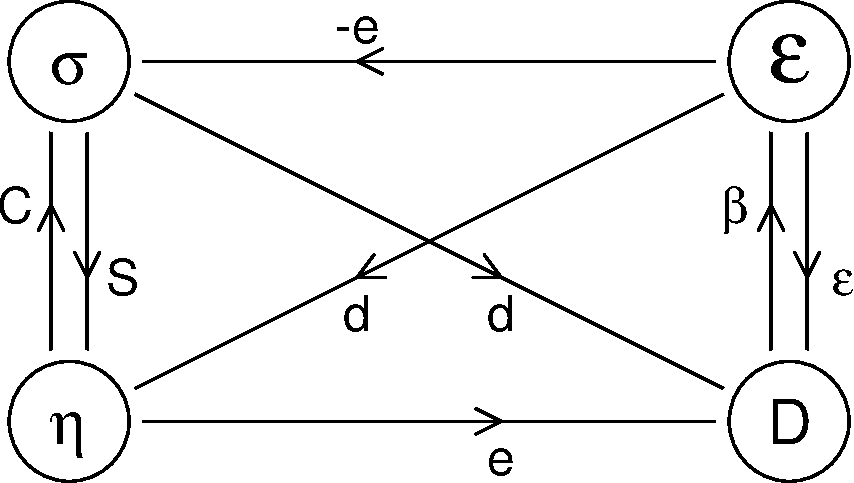
\includegraphics[width=7.6cm,angle=0]{response}
\end{center}
\caption{Definitions of response functions.}
\label{fig:response}
\end{figure}

The elastic tensors and compliances are related as inverses,
%
\beq
S^{(\E)}=(C^{(\E)})^{-1}
\eeq
%
%
\beq
S^{(D)}=(C^{(D)})^{-1} \;.
\eeq
%
The relation between $C^{(D)}$ and $C^{(\E)}$,
and between $S^{(D)}$ and $S^{(\E)}$, will be given
at the end of Sec.~\ref{sec:piezo-tens}.

Note that the compliance matrices are defined above in Voigt
notation, and in this case {\it there are factors of 2 and 4}
needed to make connection with true tensor quantities:
$S_{14}=2S_{xx,yz}$, $S_{44}=4S_{yz,yz}$, etc.  This is explained
more fully in Sec.~\ref{sec:voigt}.

Finally, note that various different definitions can be given of
the elastic constants under conditions of nonzero hydrostatic
pressure or, more generally, under nonzero stress.  In this case,
the experimentally relevant tensors (e.g., for seismic waves in
the interior of the earth) {\it do not} necessarily correspond to the ones
computed directly by \ABINIT.  For a discussion of these issues,
please see \cite{oganov}.

% %--------------------------------------------------------------
% \subsection{Dielectric tensors}
% %--------------------------------------------------------------
% \label{sec:diel}
%
% The definitions of the dielectric tensor $\eps$ and the
% inverse dielectric tensor $\beta$ are shown schematically on
% the right-hand side of Fig.~1.  These quantities can either
% be defined at fixed strain (explicitly with superscript $(\eta)$
% or implicitly if no superscript appears), or at fixed stress
% (if superscript $(\sigma)$ appears):
%
% \bigskip
%
% {\sl [TO BE WRITTEN.  WRITE IN A WAY THAT IS ROUGHLY PARALLEL TO THE
% PREVIOUS SECTION.]}
%
% \bigskip
%
% {\sl [Actually, this section is really redundant with
% Sec.~\ref{sec:eps-free-stress},
% where we already talked about $\eps^{(\sigma)}$ in a different notation.
% But maybe it doesn't matter?  Or remove earlier section?]}

%--------------------------------------------------------------
\subsection{Piezoelectric tensors}
%--------------------------------------------------------------
\label{sec:piezo-tens}

The piezoelectric tensors are defined schematically by the lines
crossing horizontally and diagonally in Fig.~(1).  (All piezoelectric
tensors are the ``proper'' ones -- see the last part of
Sec.~\ref{sec:ddbinfo} and Ref.~\cite{dv-piezo} for a discussion.)
The interpretation of the arrows is
%
\bea
\delta\eta_j &=& d_{j\alpha}\,\delta\E_\alpha
\nn
\delta D_\alpha &=& d_{j\alpha}\,\delta\sigma_j
\nn
\delta\sigma_j &=& -\,e_{j\alpha}\,\delta\E_\alpha
\nn
\delta D_\alpha &=& e_{j\alpha}\,\delta\eta_j
\;\;.
\eea
%
The first of the four equations above is sometimes said to describe
the ``converse'' piezoelectric effect, while the second one
describes the ``direct'' piezoelectric effect, and the third and/or
the fourth describe the ``inverse'' piezoelectric effect.  Thus,
one sometimes refers to $d$ as the coefficient of the ``direct
piezoelectric effect'' while $e$ (denoted as $c$ almost as often as
$e$ -- these notations are equivalent) is the coefficient of the
``inverse piezoelectric effect.''  Restating, the piezoelectric
coefficients may be defined via
%
\beq
e_{j\alpha}={\partial D_\alpha\over\partial\eta_j} \Big\vert_\E
           ={\partial P_\alpha\over\partial\eta_j} \Big\vert_\E
\qquad {\rm or} \qquad
e_{j\alpha}=-\,{\partial \sigma_j\over\partial\E_\alpha} \Big\vert_\eta
\label{eq:e-def}
\eeq
%
and
%
\beq
d_{j\alpha}= {\partial\eta_j\over\partial\E_\alpha} \Big\vert_\sigma
\qquad {\rm or} \qquad
d_{j\alpha}= {\partial D_\alpha\over\partial\sigma_j} \Big\vert_\E
           = {\partial P_\alpha\over\partial\sigma_j} \Big\vert_\E
\;\;.
\label{eq:d-def}
\eeq
%
The equivalence between the two expressions for $e$, and similarly between
the two expressions for $d$, comes from thermodynamic relations
as discussed in the Appendix of Ballato
\cite{ballato} and in Nye \cite{nye}.

The $e$ and $d$ tensors are related by
%
\beq
e_{j\alpha}=C^{(\E)}_{jk}\,d_{k\alpha}
\qquad \hbox{or, equivalently,} \qquad
d_{j\alpha}=S^{(\E)}_{jk}\,e_{k\alpha}
\;\;.
\eeq
%

One also sometimes defines tensors $g$ and $h$ via
%
\label{eq:gh-def}
\bea
\delta\eta_j &=& g_{j\alpha}\,\delta D_\alpha
\nn
\delta\E_\alpha &=& -\,g_{j\alpha}\,\delta\sigma_j
\nn
\delta\sigma_j &=& -\,h_{j\alpha}\,\delta D_\alpha
\nn
\delta\E_\alpha &=& -\,h_{j\alpha}\,\delta\eta_j
\;\;.
\eea
%
(I am not aware of any standard names for these piezoelectric
tensors.)  They are related to $e$ and $d$ via
%
\bea
g_{j\alpha}&=&\beta^{(\sigma)}_{\alpha\beta}\,d_{j\beta}
\\
\label{eq:h-relat}
h_{j\alpha}&=&\beta^{(\eta)}_{\alpha\beta}\,e_{j\beta}
\;\;.
\eea
%

The Voigt notation introduces no factors of 2 for shear components
of $e$ or $h$, but there {\it are} such factors for $d$ and $g$:
$d_{51}=2d_{xz,x}$, etc.~(see Sec.~\ref{sec:voigt}).  Also, note that
it is more common to find the indices reversed in the literature;
e.g., this piezoelectric component is more usually referred to as
`$d_{15}$'.

The relations between the elastic tensors defined at fixed $\E$
and fixed $\D$ in Sec.~\ref{sec:elas} are
%
\bea
C^{(D)}_{jk}&=&C^{(\E)}_{jk}+h_{j\alpha}\,e_{k\alpha}
\\
S^{(D)}_{jk}&=&S^{(\E)}_{jk}-g_{j\alpha}\,d_{k\alpha}
\eea
%
and between the dielectric tensors defined at fixed $\eta$
and fixed $\sigma$ in Sec.~\ref{sec:eps-free-stress} are
%
\bea
 \eps^{(\sigma)}_{\alpha\beta}&=&
 \eps^{(\eta)}_{\alpha\beta}+e_{j\alpha}\,d_{j\beta}
\label{eq:epsfs}
\\
 \beta^{(\sigma)}_{\alpha\beta}&=&
 \beta^{(\eta)}_{\alpha\beta}-g_{j\alpha}\,h_{j\beta}
\;\;.
\eea
%
Note that Eq.~(\ref{eq:epsfs}) is equivalent to Eq.~(\ref{eq:chifs}).

% %--------------------------------------------------------------
% \subsection{Electromechanical coupling constants}
% %--------------------------------------------------------------
% \label{sec:coup-factor}
%
% In the case in which there is a single kind of strain that
% couples only to a single Cartesian direction of the electric
% field, so that $C$, $\eps$, and $e$ are simply constants,
% it is conventional to define
% %
% \beq
% k^2={e^2\over C\eps}
% \eeq
% %
% which is variously known as an {\it electromechanical coupling constant}
% or a {\it piezoelectric coupling factor}.  (A case in point would be
% a tetragonal ferroelectric such as PbTiO$_3$, in which $C=C_{11}$,
% $\eps=\eps_{xx}$, and $e=e_{1x}$ for tetragonal axis along $x$.)
%
% Note that $k$ is a dimensionless measure of the strength of the
% piezoelectric coupling.  The meaning of $k$ can also be
% seen by ...    instability ... efficiency ... {\sl [ FINISH ]}
%
% In the general case, it is possible to compute the electromechanical
% coupling tensor as
% %
% \beq
% k_{j\alpha}=(C^{-1/2})_{jk}\;(\eps^{-1/2})_{\alpha\beta}\;e_{k\beta}
% \;\;.
% \eeq
% %
% In a simple case, like that of tetragonal PbTiO$_3$, this tensor may
% have just a single non-zero element, which will be the $k$ discussed
% above.  However, in general, one can decompose it into ``active
% channels'' via the singular value decomposition
% %
% \beq
% k=U\,\kappa\,V^\dagger
% \eeq
% %
% where $U$ is a 6$\times$6 unitary matrix, $\kappa$ is a positive
% real diagonal 3$\times$6 matrix (that is, the only non-zero
% elements are $\kappa_{11}$, $\kappa_{22}$, $\kappa_{33}$, normally
% abbreviated to just $\kappa_1$ etc., and these are all real and
% positive), and $V$ is a 3$\times$3 unitary matrix.  There are
% standard mathematical library subroutines for doing this
% decomposition.  Then the diagonal elements of $\kappa$, which are
% known as the ``singular values,'' are the relevant
% electromechanical coupling constants.  It may also be of interest
% to report, for each $\kappa_i$, the corresponding mechanical strain
% channel (i.e., print out the $i$'th column of of $U$) and electric
% field channel (i.e., print out the $i$'th column of of $V$) that
% are electromechanically coupled by $\kappa_i$.
%
% %==============================================================
% \section{More on phonon modes and lattice dielectric response}
% %==============================================================
% \label{sec:ir-phonons}
%
% %==============================================================
% \section{Thermodynamic energy functions}
% %==============================================================
% \label{sec:thermo}
%
% {\sl To be written.}

%==============================================================
\section{Voigt notation}
%==============================================================
\label{sec:voigt}

%--------------------------------------------------------------
\subsection{Basic formulation}
%--------------------------------------------------------------

There are two systems that are commonly in use to index quantities
that depend on strains or stresses: the ``true tensor notation'' in which
all Cartesian indices are written explicitly, and the ``Voigt notation''
in which a reduced index is used:
$xx\rightarrow 1$, $yy\rightarrow 2$, $zz\rightarrow 3$,
$yz\rightarrow 4$, $xz\rightarrow 5$, $xy\rightarrow 6$.
The stress elements are defined simply by making this index
replacement:
%
\bea
\label{eq:voigt-sig}
&& \sigma_1=\sigma_{xx} \qquad
   \sigma_4=\sigma_{yz} \nonumber \\
&& \sigma_2=\sigma_{yy} \qquad
   \sigma_5=\sigma_{xz} \\
&& \sigma_3=\sigma_{zz} \qquad
   \sigma_6=\sigma_{xy} \nonumber
\eea
%
However, the {\it strain elements have factors of two inserted in
the definition of the shear elements}:
%
\bea
\label{eq:voigt-eta}
&& \eta_1=\eta_{xx} \qquad
   \eta_4=2\eta_{yz} \nonumber \\
&& \eta_2=\eta_{yy} \qquad
   \eta_5=2\eta_{xz} \\
&& \eta_3=\eta_{zz} \qquad
   \eta_6=2\eta_{xy} \nonumber
\eea

The context here is that $\eta$ is a symmetric
tensor, i.e., $\eta_{xy}=\eta_{yx}$, defined via
$\eta_{\alpha\beta}=\half(u_{\alpha,\beta}+u_{\beta,\alpha})$.
Here $u_{\alpha,\beta}=\partial u_\alpha/\partial x_\beta$ is
the unsymmetrized tensor defined in term of spatial derivatives
$\partial/\partial x_\beta$ of the medium displacement $u_\alpha$.
Thus, we could
alternatively have written $\eta_6=\eta_{xy}+\eta_{yx}$, etc.

The reason for the introduction of these factors of 2 is explained
very nicely in the book by Nye, Ref.~\cite{nye}
(see, e.g., Secs.~VII.2-3 and VIII.2 therein).  I give a brief
discussion based on the thermodynamic energy function
$H$ of Sec.~\ref{sec:notation}.  The change $dH$ of the energy
should be the same in both frameworks.  In the true tensor
framework, $H$ is a a function of 9 variables, and we can write
%
\beq
dH= \sigma_{xx} \, d\eta_{xx} + ...
+ \sigma_{yz} \, d\eta_{yz} + ...
+ \sigma_{zy} \, d\eta_{zy} + ...
\eeq
%
where each `$...$' indicates two more terms obtained by cyclic
permutation of $(xyz)$.
On the other hand, in the Voigt framework, the same $dH$ can
be written as a sum of only six terms as
%
\beq
dH= \sigma_1 \, d\eta_1 + ...
+ \sigma_4 \, d\eta_4 + ...
\eeq
%
where each `$...$' indicates two more terms obtained by cyclic
permutation $(123)$ or $(456)$.
Comparing these two equations, which must be equal, and using that
$\eta_{yz}=\eta_{zy}$, it is clear that a factor of two must be inserted
into the defining connection either between $\sigma_{yz}$ and $\sigma_4$,
or else between $\eta_{yz}$ and $\eta_4$.  The Voigt notation arises
from making the second choice, i.e., Eqs.~(\ref{eq:voigt-sig}) and
(\ref{eq:voigt-eta}).

In practice, this means that if you want to introduce a Voigt strain
$\eta_6=t$ into an \ABINIT\ calculation (say in order to check, by
finite differences, the computation of the stress or elastic tensor),
then one should set $\eta_{xy}=\eta_{yx}=t/2$ when constructing the
unit cell.  For example, if the original cell vectors describe
a simple cubic lattice, then the new lattice vectors could be
${\bf a}_1'=a(1,t/2,0)$,
${\bf a}_2'=a(t/2,1,0)$,
and ${\bf a}_3'=a(0,0,1)$;
or they could be
${\bf a}_1'=a(1,t,0)$,
${\bf a}_2'=a(0,1,0)$,
and ${\bf a}_3'=a(0,0,1)$; etc.
(In the first case, $u_{x,y}=u_{y,x}=t/2$;
in the second case, $u_{x,y}=0$ and $u_{y,x}=t$; in both cases,
$\eta_{xy}=t/2$ and $\eta_6=t$.)
Then, if $H$ is expanded in powers of $t$, the coefficient of the
linear term is just $\sigma_6$, the coefficient of the
quadratic term is just $C_{66}$, etc.

%--------------------------------------------------------------
\subsection{Systematics}
%--------------------------------------------------------------

We can understand when to insert, or not to insert, factors of 2
in the relations between Voigt and Cartesian notations by following
the following rules:

\begin{itemize}

\item
Any inserted factor of two makes the Voigt object larger: $Q_{...4...}=
2Q_{...yz...}$

\item
If there is a factor of $\eta$ in the numerator of a derivative,
{\it do insert} a factor of 2 for each shear component.

\item
If there is a factor of $\sigma$ in the numerator of a derivative,
no factors are needed.

\item
If there is a derivative with respect to $\eta$, no factors are needed.

\item
If there is a derivative with respect to $\sigma$, {\it do insert}
a factor of 2 for each shear component.

\end{itemize}

\noindent
Thus, there is no need to insert factors of two when interpreting
most of the objects we have introduced, including $\sigma$, $C$, $e$,
$\Lambda$, and $\Gamma$.  However, we {\it do} need factors for $S$;
since $S_{ij}=d\eta_i/d\sigma_j$, we need $S_{14}=2S_{xx,yz}$,
$S_{44}=4S_{yz,yz}$, etc.
As for the piezoelectric
tensors, it is clear from Eqs.~(\ref{eq:e-def}-\ref{eq:h-relat})
and the rules given above that factors of 2
{\it are} needed for $d$ and $g$, but not for $e$ and $h$.

Finally, in the linear-response calculation, one needs to calculate
and store objects such the first-order derivatives of Bloch
wavefunctions with respect to strains, i.e., $d\vert u_{n{\bf k}}\rangle
/d\eta_j$.  This is a derivative with respect to strain, so by
the above rules, there is no need to worry about a factor of two
in the definition of this object.

%--------------------------------------------------------------
\subsection{A word about terminology}
%--------------------------------------------------------------

Nye (Ref.~\cite{nye}) refers to the arrays of Voigt elements as
``matrices'' while the arrays of Cartesian-labeled elements are
called ``tensors.'' In his terminology, the term ``tensor'' is
reserved for objects that transform under rotations by the
application of the associated 3$\times$3 rotation matrix to each
Cartesian index.  Thus, for example, the rotated piezoelectric
tensor is given by
%
\beq
e_{\beta\gamma,\alpha}'= R_{\beta\mu} \, R_{\gamma\nu}\,
R_{\alpha\tau}\,e_{\mu\nu,\tau}
\eeq
%
where $R$ is the rotation matrix and there are implicit sums over
repeated indices.  Since the the $6\times3$ matrix
of $e_{j\alpha}$ elements in the Voigt notation does {\it not}
transform in a similar way, Nye takes pains to call the
Voigt $e_{j\alpha}$ a ``matrix'' and not a ``tensor.''

While Nye's point is very well taken, the habit of
referring to the Voigt elements $e_{j\alpha}$ as elements of the
``piezoelectric tensor'' is by now rather widely ingrained, and in my
opinion it is rather too pedantic to insist on the narrow definition.
In these notes, therefore, I generally use the term ``tensor'' to
refer indiscriminately to either the Voigt or the fully Cartesian
notations.  However, in deference to Nye, I do sometimes use the
extended phase ``true tensor notation'' to refer to the fully
Cartesian notation.


%==============================================================
\section{Summary}
%==============================================================

As of January 2004, the calculation of the following quantities
has been implemented for the proposed update of \ANADDB\ to version 4.3:

\begin{itemize}
%
\item All six ``bare'' tensors $K$, $C$, $\chi$,
$\Lambda$, $Z$ and $e$, Sec.~\ref{sec:notation}.
%
\item The clamped-ion compliance tensor $S$ of Sec.~\ref{sec:compliance}.
%
\item The displacement-response internal-strain tensor
$\Gamma$ of Sec.~\ref{sec:internal}.
%
\item The relaxed-ion elastic, dielectric, and piezoelectric
tensors ($\wt{C}$, $\wt{\chi}$, and $\wt{e}$) of Sec.~\ref{sec:formulation},
and the relaxed-ion compliance tensor $S^{(\E)}$ of Sec.~\ref{sec:elas}.
%
\end{itemize}

\noindent
It is our intention to include the ability to calculate additional
tensors, including many of the ones defined in Secs.~\ref{sec:elas}
and \ref{sec:piezo-tens}, in a future release of the \ANADDB\ module
of \ABINIT.


%==============================================================
\begin{thebibliography}{99}
%==============================================================

\bibitem{abi} {\sf ABINIT} is a common project of the
Universit\'{e} Catholique de Louvain,
Corning Incorporated, and other contributors (https://www.abinit.org).
X. Gonze, J.-M. Beuken, R. Caracas, F. Detraux, M. Fuchs, G.-M. Rignanese,
L. Sindic, M. Verstraete, G. Zerah, F. Jollet, M. Torrent, A. Roy,
M. Mikami, Ph. Ghosez, J.-Y. Raty, D.C. Allan,
Comput. Mater. Sci. {\bf 25}, 478-492 (2002).

\bibitem{oganov}
A set of notes on elastic constants can be found in the file
{\sl `elasticity-oganov.pdf'} written by A.~Oganov and located in
the {\sl /Infos} subdirectory of the {\sf ABINIT} distribution.

\bibitem{lines} M. E. Lines and A. M. Glass, {\it Principles and
Applications of Ferroelectrics and Related Materials,} (Clarendon
Press, Oxford, 1977).

\bibitem{nye} J. F. Nye, {\it Physical properties of crystals}
(Oxford U.P., Oxford 1985).

\bibitem{ballato} A.~Ballato, IEEE Transac. Ultrason. Ferro. and
Freq. Control {\bf 42}, 916 (1995).

\bibitem{waghmare} U.~Waghmare, unpublished.

\bibitem{baroni87} S.~Baroni, P. ~Giannozzi and A.~Testa,
Phys. Rev. Lett. {\bf 78}, 1861 (1987).

\bibitem{degir91} P. Giannozzi, S. de Gironcoli, P. Pavone, and S. Baroni,
Phys. Rev. B {\bf 43}, 7231 (1991).

\bibitem{gonze95a} X.~Gonze, Phys. Rev. A {\bf 52}, 1096 (1995).

\bibitem{gonze97a}  X.~Gonze,
Phys. Rev. B {\bf 55}, 10337 (1997).

\bibitem{gonze97b} X.~Gonze and C. ~Lee, Phys. Rev. B {\bf 55}, 10355 (1997).

\bibitem{rmp-baroni} S. Baroni, S. de Gironcoli, A. Dal Corso,
and P. Giannozzi, Rev. Mod. Phys. 73, 515 (2001).

\bibitem{ksv} R.D.~King-Smith and D.~Vanderbilt,
Phys. Rev. B {\bf 47}, 1651 (1993).

\bibitem{rmp-resta} R. Resta, Rev. Mod. Phys. 66, 899 (1994).

\bibitem{nunes01} R. W. Nunes and X. Gonze, Phys. Rev. B {\bf 63}, 155107
(2001).

\bibitem{souza-ef} I.~Souza, J.~\'I\~niguez, and D.~Vanderbilt,
Phys. Rev. Lett. {\bf 89}, 117602 (2002).

\bibitem{dv-piezo} D. Vanderbilt, J. Phys. Chem. Solids {\bf 61}, 147 (2000).

\end{thebibliography}



\end {document}
